\documentclass{ezb}
\usepackage[]{todonotes}
\usepackage{amsmath}
\usepackage{gensymb}
\usepackage{wrapfig}
\usepackage{longtable}
\usepackage{amssymb}
\usepackage[colorlinks,        	% Links ohne Umrandungen in zu wählender Farbe
   linkcolor=black,   			% Farbe interner Verweise
   filecolor=black,   			% Farbe externer Verweise
   citecolor=black    			% Farbe von Zitaten
]{hyperref}
\usepackage{booktabs}

\renewcommand{\thesubsection}{\alph{subsection}}
\begin{document}

% \maketitle{Nummer}{Abgabedatum}{Tutor-Name}{Gruppennummer}
%           {Teilnehmer 1}{Teilnehmer 2}{Teilnehmer 3}
\maketitle{05.06.15}{Udo Frese}{1}{Annika Ofenloch - 2992807 - ofenloch@uni-bremen.de}{Frank Ihle - 3010158 - fihle@uni-bremen.de}{Simon Schirrmacher - 4000884 - simons@informatik.uni-bremen.de}{Noshaba Cheema - ncheema@uni-bremen.de}

%-------Text-Start------------------------------------------
\section{Ballspiele I (10 Punkte)}
\begin{lstlisting}[language=C++]

HoughCircle::Parameters::Parameters()
 :rMin(10), rMax(15), sobelThreshold(7), houghThreshold(7), radiusHoughThreshold(0), localMaxRange(100)
{
	// so that findBestRadius and other functions do not have a buffer overflow
	if (rMin < 0) rMin = 0;
	if (rMax < 0) rMax = 0;
}

void HoughCircle::create (int width, int height, const Parameters &param)
{
    // implement (2P)
	imgWidth = width;
	imgHeight = height;
	// + 2 * RMAX to not to exceed edges of image
	houghImgWidth = width + (param.rMax << 1);
	houghImgHeight = height + (param.rMax << 1);
	// create dummy image to determine step size
	Mat_<ushort> dummyImg(houghImgHeight, houghImgWidth);
	houghImgWidthStep = dummyImg.step[0] / dummyImg.step[1];
	//deallocate memory
	dummyImg.release();
	// init sobel angle LUT
	sobelTab.clear();
	float angle, ang;
	for (int y = -128; y < 128; ++y) for (int x = -128; x < 128; ++x) {
		ang = atan2(y, x);
		angle = fabs(ang) * 255.0f / M_PI; // normalize and discretize angle
		sobelTab.push_back(SobelEntry((int)round(sqrt(sq(x) + sq(y))), (int) round(angle), cos(ang), sin(ang)));
	}
	// init relative address LUT
	relativeAddressForAngleAndR.clear();
	int dX, dY;
	for (int angle = 0; angle < Parameters::NR_OF_ORIENTATIONS; ++angle) for (int r = 0; r <= param.rMax; ++r){
		dX = r * cos(angle);
		dY = r * sin(angle);
		relativeAddressForAngleAndR.push_back(dX + houghImgWidthStep * dY);
	}
	// error handling
	assertSobelTab();
    assertRelativeAddressForAngleAndRTab();
}

void HoughCircle::addPointToAccumulator (ushort* houghImgOrigin, int x, int y, int sobelCoded) const
{
    // implement (1P)
	int relAddr;
	for (int r = param.rMin; r <= param.rMax; ++r) {
		relAddr = relativeAddressForAngleAndR[sobelTab[sobelCoded].angle*(param.rMax+1)+r];
		// along normal
		houghImgOrigin[y * houghImgWidthStep + x + relAddr]++;
		// opposed normal
		houghImgOrigin[y * houghImgWidthStep + x - relAddr]++;
	}
}
\end{lstlisting}

\newpage
\begin{lstlisting}[language=C++]
void HoughCircle::hough (Mat_<ushort>& houghImg, const Mat_<ushort>& sobelImgPrev, const Mat_<ushort>& sobelImg) const
{
    // implement (1P)
	// error handling
	assert("sobelPrev and sobel must have the same size" && sobelImgPrev.rows == sobelImg.rows && sobelImgPrev.cols == sobelImg.cols);
	int sobelLen, sobelLenPrev;
	// calculate origin of hough image
	ushort* origin = houghImg.ptr<ushort>(param.rMax)+param.rMax;
	// for more performance
	#pragma omp for
	for (int y = 0; y < sobelImg.rows; ++y) {
		for (int x = 0; x < sobelImg.cols; ++x) {
			// calculate sobel length of previous sobelImg
			sobelLenPrev = sobelTab[sobelImgPrev(y, x)].length;
			// calculate sobel length of sobelImg
			sobelLen = sobelTab[sobelImg(y, x)].length;
			// wasn't sure if > or >= since in line 97 in the header "exceed" is written
			// but in line 22 it says it ignore every value below sobelThreshold
			if ((sobelLen - sobelLenPrev) > param.sobelThreshold)
				addPointToAccumulator(origin, x, y, sobelImg(y,x));
		}
	}
}


bool HoughCircle::isLocalMaximum (const Mat_<ushort>& houghImg, int xC, int yC) const
{
    // implement (2P)
	const ushort *hLine = nullptr;
	const ushort center = houghImg.ptr<ushort>(yC)[xC];
	// [+localMaxRange,-localMaxRange]
	for (int dy = -param.localMaxRange; dy <= param.localMaxRange; ++dy) {
		// check if no edge exceeding
		if (yC + dy >= 0 && yC + dy < houghImgHeight){
			hLine = houghImg.ptr<ushort>(yC);
			hLine = houghImg.ptr<ushort>(yC + dy);
			for (int dx = -param.localMaxRange; dx <= param.localMaxRange; ++dx) {
				// check if no edge exceeding and return false if greater value was found
				if (xC + dx >= 0 && xC + dx < houghImgWidth &&
					center < hLine[xC + dx])
					return false;
			}
		}
	}
	return true;
}

\end{lstlisting}
\newpage
\begin{lstlisting}[language=C++]
int HoughCircle::findBestRadius (const Mat_<ushort>& sobelImg, int xC, int yC, int& bestR) const
{
    // implement (2P)

	// init hough R
	std::vector<int> houghR;
	for (int r = 0; r <= param.rMax; ++r)
		houghR.push_back(0);

	// increase houghR at r if fitting value was found
	SobelEntry s;
	int r; float d;
	for (int dY = -param.rMax; dY <= param.rMax; dY++)
		for (int dX = -param.rMax; dX <= param.rMax; dX++) {
			// check for edge exceeding
			if (xC + dX >= 0 && xC + dX < sobelImg.cols &&
				yC + dY >= 0 && yC + dY < sobelImg.rows) {
				s = sobelTab[sobelImg(yC + dY, xC + dX)];
				// calculate radius
				r = fabs(s.cosAngle *dX + s.sinAngle*dY);
				d = fabs(-s.sinAngle*dX + s.cosAngle*dY);
				if (d <= 1 && s.length > param.sobelThreshold && r <= param.rMax)
					houghR[r]++; // increase if good value
			}
		}

	// find best radius and valueR
	bestR = param.rMin;
	int bestVal = 0;
	for (int r = param.rMin; r <= param.rMax; r++) {
		if (houghR[r]>houghR[bestR]) { 
			bestR = r; 
			bestVal = houghR[r];
		}
	}

	return bestVal;
}


void HoughCircle::extractFromHoughImage (vector<Circle>& circles, const Mat_<ushort>& houghImg, const Mat_<ushort>& sobelImg) const
{
    // implement (1P)
	circles.clear();
	const ushort* pLine = nullptr;
	int bestR;
	int valueR;
	// starts at +RMAX and ends at end-RMAX because the hough room is 2*RMAX in both dimensions
	// greater than the original image
	for (int y = param.rMax; y < houghImgHeight - param.rMax; ++y) {
		pLine = houghImg.ptr<ushort>(y);
		for (int x = param.rMax; x < houghImgWidth - param.rMax; ++x) {
			// find a high enough entry as center
			if (pLine[x] >= param.houghThreshold && isLocalMaximum(houghImg, x, y)) {
				valueR = findBestRadius(sobelImg, x, y, bestR);
				// entry has to be at least radiusHoughThreshold (line 25 in header)
				if (valueR >= param.radiusHoughThreshold)
					// calculate hough img coordinated to original img coordinates
					circles.push_back(Circle(x - param.rMax, y - param.rMax, bestR, pLine[x], valueR));
			}
		}
	}
}
\end{lstlisting}
\newpage
\begin{lstlisting}[language=C++]

void HoughCircle::findCircles (vector<Circle> &circles, Mat_<ushort>& houghImg, const Mat_<ushort>& sobelPrev, const Mat_<ushort>& sobel) const
{
    // implement (1P)
	// error handling
	assert("sobel images must be the same size" && sobel.cols == sobelPrev.cols && sobel.rows == sobelPrev.rows);
	circles.clear();
	// create hough image if not allocated
	if (houghImg.empty())
		houghImg = createHoughImage();
	#pragma omp parallel
	{
		// apply hough transform
		hough(houghImg, sobelPrev, sobel);
	}
	// create circle out of transform
	extractFromHoughImage(circles, houghImg, sobel);
}

\end{lstlisting}



\newpage
\section{Tag des Modellbaus (4 Punkte)}
Unter Verwendung der Bildverarbeitung soll ein Zeppelinmodell, autonom eine vordefinierte Route über einer Wiese fliegen.\\
\linebreak
Um die Orientierung des Zeppelins auf der Wiese zu ermöglichen, werden Markierungen auf der Wiese ausgelegt, welche als Wegpunkte zu interpretieren sind. Die Markierungen haben die Form eines Pfeils und geben somit Aufschluss über die zu fliegende Richtung.Um diese erfassen zu können, wird unter dem Zeppelin eine Kamera angebracht, die senkrecht nach unten filmt (siehe Abb. \ref{fig1}).\\ 
\begin{figure}[h]
	\centering
  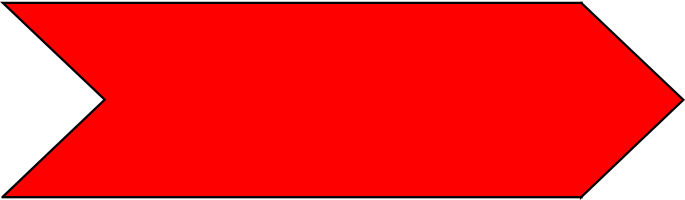
\includegraphics[scale=0.7]{richtungspfeil.png}
	\caption{Beispiel eines Markierungspfeils für die Bewegungsvorgabe des Zeppelins.}
	\label{fig1}
\end{figure}
\linebreak
\begin{wrapfigure}{r}{0.2\textwidth}

\includegraphics[width=0.15\textwidth]{regelkreis.png}
\caption{\label{fig:kreis}Start-Markierung}
\end{wrapfigure}
Für den Start wird eine besondere runde Markierung eingesetzt. Zu Beginn des Rundflugs befindet sich der Zeppelin direkt auf dem Kreis und schwebt beim Start senkrecht in die Höhe.\\ Anhand der Größe des Kreises, welche mit zunehmender Höhe immer weiter abnimmt, kann der Zeppelin feststellen, ob bereits die gewünschte Höhe erreicht wurde.\\
\linebreak
Ist diese Höhe erreicht, orientiert sich der Zeppelin an einem Strich, welcher vom Kreisrand bis zur Mitte des Kreises gezeichnet ist. Dieser Strich gibt die initiale Richtung an (siehe Abb. \ref{fig:kreis}). Jede durch die Markierungen definierte Richtung zeigt auf den Mittelpunkt (Schwerpunkt) der nächsten Markierung. Die Markierungen, welche die Wegpunkte beschreiben, sind einfarbig gefärbt und es ist eine bestimmte, sich wiederholende, Farbfolge definiert, wodurch bei mehreren erkannten Markierungen die nächst folgende ausgewählt werden kann (siehe Abb. \ref{fig:farbfolge}).\\
\begin{figure}[h]
	\centering
  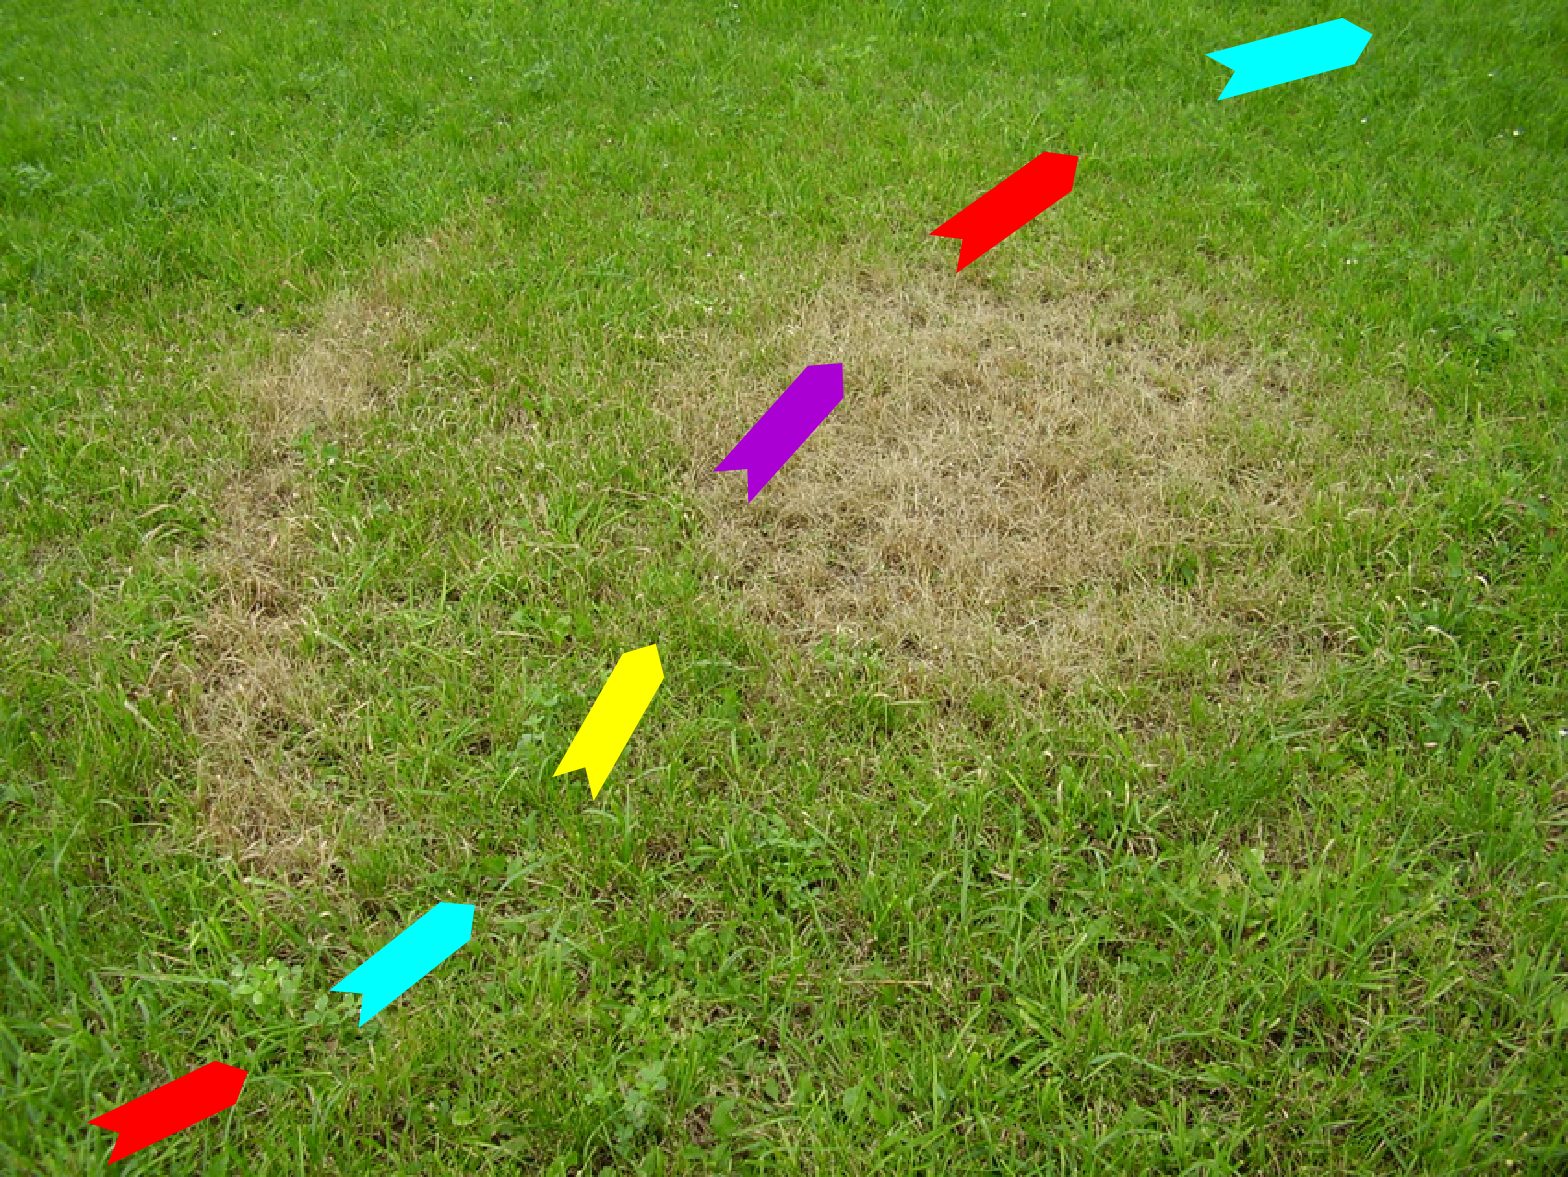
\includegraphics[scale=0.5]{richtungspfeileAufWieseBunt.png}
	\caption{Beispiel einer Farbfolge}
	\label{fig:farbfolge}
\end{figure}
\linebreak
Zudem sind sie so geformt, dass nicht die gesamte Markierung im Bild erfasst sein muss, um die vorgegebene Richtung zu erfassen. Um dies zu erreichen, sind Anfang und Ende des Pfeils so geformt, dass diese eindeutig erkennbar sind (siehe Abb. \ref{fig1}).\\ 
\linebreak
Wird eine Markierung erkannt, richtet sich der Zeppelin entsprechend seine Vorgabe auf dem Boden aus. Von diesem Markierungspfeil werden die Trägheitsachsen gebildet und anhand der Pfeilspitzen die Bewegungsrichtung vorgegeben. Mit Hilfe dieser Trägheitsachse und der Geraden, auf der sich das Flugobjekt vorwärts bewegt, lässt sich über trigonometrische Funktionen den Winkel ermitteln, den es einzustellen gilt, um die Bewegungsrichtung zu ändern. Ist bereits eine neue Markierung im Blickfeld (neu bedeutet: in der oberen Bildhälfte), dann soll deren Mittelpunkt angesteuert werden. Wenn nicht wird entsprechend der Vorgaben der zuletzt gefundenen Markierung geradeaus geflogen. Erst wenn die angesteuerte Markierung in der unteren Bildhälfte liegt (also hinter dem Zeppelin), wird auf die nächst verfügbare navigiert.\\
\linebreak 
Beim Einbau der Kamera ist davon auszugehen, dass deren vertikalen und horizontalen Achsen nicht senkrecht bzw. parallel zur Bewegungsrichtung verlaufen, wofür die Kamera vor Inbetriebnahme zunächst kalibriert werden muss.\\
\linebreak
Da nach diesen Vorgaben oft nachgesteuert wird, empfiehlt es sich die Bewegungsvorgabe mit einem Regler anzusteuern, um eventuellen Schwingzuständen entegegen zu wirken.\\ 
\linebreak
Für die Landung wird ein weiterer Kreis als Markierung eingesetzt, in welchen jedoch kein Strich eingezeichnet sein muss. Es kann sich bei diesem Kreis auch um den selben Kreis handeln, von dem aus gestartet wurde. Wird dieser Kreis erkannt, sinkt der Zeppelin senkrecht.

\section{Spargel, Bildverarbeitung und soziale Realität (1 Bonuspunkt)}
Qualitätsmerkmale, wie beispielsweise die Farbe (bzw. Verfärbung), Vollständigkeit als auch die Form, lassen sich durch Angestellte schnell kontrollieren. Es kann demnach überprüft werden, ob der Spargel von Schädlingen befallen, verfault, verschmutzt, abgebrochen, krumm oder hohl ist.\\ 
\linebreak 
Bei den Merkmalen wie, Länge und Durchmesser reicht das Augenmaß nicht immer aus. Insbesondere beim Durchmesser ist es schwierig die präzise Unterscheidung in die einzelnen Güteklassen durchzuführen, da es sich hier oft um Abweichungen von Millimetern handelt. Der Angestellte hat demnach Schwierigkeiten zu beurteilen, ob der Spargel einen Durchmesser von 8 oder 10 mm aufweist (Mindestdurchmesser bei Klasse I: 10 mm, bei Klasse II: 8 mm). \\ 
\linebreak
Auch die Länge des Spargels kann durch Angestellte nicht immer mit bloßen Augenmaß richtig eingeschätzt werden. Sobald sich die Länge in der Nähe von Grenzwerten befindet, ist es besonders wichtig, die exakte Länge zu bestimmen. Wenn der Spargel zum Beispiel 17,3 cm lang ist, zählt er zum langen und nicht mehr zum kurzen Spargel. Ein Angestellter würde dies gegebenenfalls nicht sehen und den Spargel falsch zuordnen. Es ist in solchen Fällen also wichtig, wenn sich der Angestellte nicht sicher ist, den Spargel an ein Bildverarbeitungssystem weiter zu geben. Dort kann der genaue Durchmesser als auch die Länge des Spargels ermittelt werden. Ansonsten ist der Angestellte in der Lage mit bloßem Auge erkennen zu können, ob es sich beispielsweise, um ein sehr kleines Exemplar handelt.

%-------Text-End------------------------------------------
\end{document}

